%% Based on:

%%%%%%%%%%%%%%%%%%%%%%%%%%%%%%%%%%%%%%%%%
% a0poster Portrait Poster
% LaTeX Template
% Version 1.0 (22/06/13)
%
% The a0poster class was created by:
% Gerlinde Kettl and Matthias Weiser (tex@kettl.de)
% 
% This template has been downloaded from:
% https://www.latextemplates.com/template/a0poster-portrait-poster
%
% License:
% CC BY-NC-SA 3.0 (http://creativecommons.org/licenses/by-nc-sa/3.0/)
%
%%%%%%%%%%%%%%%%%%%%%%%%%%%%%%%%%%%%%%%%%


%----------------------------------------------------------------------------------------
%	PACKAGES AND OTHER DOCUMENT CONFIGURATIONS
%----------------------------------------------------------------------------------------

\documentclass[a0,landscape]{a0poster}

\usepackage{multicol} % This is so we can have multiple columns of text side-by-side
\columnsep=100pt % This is the amount of white space between the columns in the poster
\columnseprule=3pt % This is the thickness of the black line between the columns in the poster

\usepackage[svgnames]{xcolor} % Specify colors by their 'svgnames', for a full list of all colors available see here: http://www.latextemplates.com/svgnames-colors

%\usepackage{newtxtext} % Use the times font for text, newer flavor
\usepackage{helvet}
\renewcommand{\familydefault}{\sfdefault} % sans serif font

\usepackage{graphicx} % Required for including images
\graphicspath{{img/}} % Location of the graphics files
\usepackage{booktabs} % Top and bottom rules for table
\usepackage[font=small,labelfont=bf]{caption} % Required for specifying captions to tables and figures
\usepackage{amsfonts, amsmath, amsthm, amssymb} % For math fonts, symbols and environments
\usepackage{wrapfig} % Allows wrapping text around tables and figures

\usepackage{physics}
\usepackage[T1]{fontenc}
\usepackage[utf8]{inputenc}
\usepackage{setspace}

\usepackage{bbm}

\usepackage[top=1cm,right=2.8cm,bottom=1cm,left=2.6cm]{geometry}

%\usepackage{lipsum}

\usepackage[safeinputenc,doi=false,url=false,backend=biber]{biblatex}
\addbibresource{bib/main.bib}

% %% https://tex.stackexchange.com/a/366170
% \makeatletter
% \renewenvironment{abstract}{%
%   \begin{center}%
%     {\bfseries \large\abstractname\vspace{\z@}}
%   \end{center}%
%   \quotation
% }
% \makeatother

%----------------------------------------------------------------------------------------
% FROM tex/lib.tex
%----------------------------------------------------------------------------------------
% TODO: DRY
\newcommand{\term}[1]{\emph{#1}}
\newcommand{\idop}{\mathbbm{1}}           % Identity operator
\newcommand{\hilb}[1]{\mathcal{#1}}       % Hilbert space
\newcommand{\setof}[1]{\left\{#1\right\}}
\newcommand{\ox}{\otimes}
%
%% Allows better formatting than \underset
%% https://tex.stackexchange.com/a/130553
\DeclareMathOperator*{\repr}{\equiv}      % represented in a basis, or "has components..."
%
\renewcommand{\op}{\hat}                  % overwriting physics \op = \ketbra
\newcommand{\eqbydef}{\coloneqq}
%\newcommand{\eqbydef}{\triangleq}
\newcommand{\superop}{\mathcal}
%
\newcommand{\smallback}{\hspace{-0.115em}}
\newcommand{\largeback}{\hspace{-0.365em}}
%
\newcommand{\dket}[1]{\left.\left| #1 \right\rangle\smallback\right\rangle}
\newcommand{\Dket}[1]{\left.\left| #1 \right\rangle\largeback\right\rangle}
% and similar...
\newcommand{\dbra}[1]{\left\langle\smallback\left\langle #1 \right|\right.}
\newcommand{\dbraket}[2]{\left\langle\smallback\left\langle #1 \middle| #2 \right\rangle\right.}
\newcommand{\bradket}[2]{\left.\left\langle #1 \middle| #2 \right\rangle\smallback\right\rangle}
\newcommand{\dbradket}[2]{\left\langle\smallback\left\langle #1 \middle| #2 \right\rangle\smallback\right\rangle}
\newcommand{\dketdbra}[2]{\left| #1 \left\rangle\smallback\left\rangle \smallback \right\langle\smallback\right\langle #2 \right|}

\newcommand{\pwspace}{\hilb{H}_T \ox \hilb{H}_S}

%\renewcommand{\abstractname}{\large Abstract} % abstract hacks

\begin{document}
%----------------------------------------------------------------------------------------
%	POSTER HEADER 
%----------------------------------------------------------------------------------------
\begin{minipage}[c]{0.60\linewidth}%
\Huge\color{NavyBlue}\textbf{Quantum Time: Page-Wootters and Detector Models}
  \color{Black}
  \\[0.5cm]
  \Large \textbf{Guido De Rosa, Andreas Ruschhaupt} |
  \Large University College Cork, Department of Physics | % University/organization
  \texttt{gderosa@umail.ucc.ie}
\end{minipage}%
%
\begin{minipage}[c]{0.40\linewidth}
  \vspace{1.5cm}\hspace{0cm}
\includegraphics[width=11cm]{ucc_logo.pdf}\\[0.0cm]
\end{minipage}

%\vspace{1cm} % A bit of extra whitespace between the header and poster content

%----------------------------------------------------------------------------------------

\begin{multicols}{3} 

%----------------------------------------------------------------------------------------
%	ABSTRACT
%----------------------------------------------------------------------------------------

\color{Navy} % Navy color for the abstract

\section*{\large Abstract}
%\noindent % abstract hacks
We compare the Page and Wootters (PaW) model of quantized time
(see \cite{PageWootters, Lloyd:Time} for an outline of the theory,
or \cite{Moreva:illustration, Moreva_position} for experimental realizations)
with detection models based on absorption and loss of normalization
by a complex potential \cite{RuschhauptAbsorption}. We show that the prediction
of the Page--Wootters mechanism and of such detector model are compatible both in terms
of the state evolution and
the probability distribution of
time-of-arrival at a particular state.
We do this by both ``plugging-in``
the imaginary absorption term (for detectors that strongly alter the system dynamics)
\emph{and} considering a weaker absorption regime, where the PaW model makes
the imaginary term in the Hamiltonian unnecessary. We emphasize that the probability
of detection in time is a \emph{conditional}
probability, in the Bayesian \cite{Maccone:QMOT} sense.


%\end{abstract}

\setlength{\parindent}{1.5em} % Default is 15pt.

%\color{SaddleBrown} % SaddleBrown color for the introduction

\large

\color{DarkSlateGray} % DarkSlateGray color for the rest of the content

\section*{Detector model: Complex potential of minimal uncertainty}

For a two-level system, if we consider \cite{RuschhauptAbsorption}:
\begin{equation}\label{eq:complexpot}
  \mathcal{K} = \hat{H} - i\hat{D} \repr
    \left[\begin{matrix}0 & 1\\1 & 0\end{matrix}\right] -
    i \left[\begin{matrix}0 & 0\\0 & \gamma \end{matrix}\right]
    \,\text{,}
\end{equation}
with an initial state of $\ket{0}$
(or $\left[\begin{matrix}1\\0\end{matrix}\right]$ in matrix form),
minimal time-energy uncertainty is found with $\gamma = \sqrt{2}/2$.

Time-of-arrival at state $\ket{1}$:
\begin{center}\vspace{1cm}
  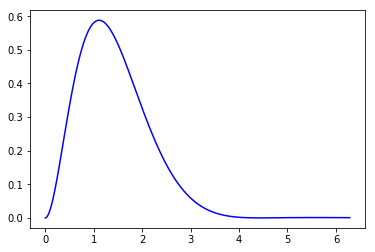
\includegraphics[width=0.4\linewidth]{2ldetect/toa-cont.png}
  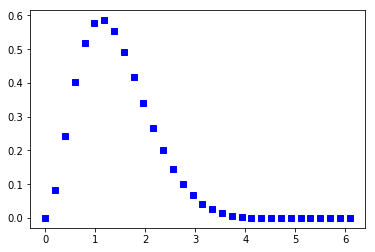
\includegraphics[width=0.4\linewidth]{2ldetect/toa-pw.png}
  \captionof{figure}{
    \label{fig:toa}
    \color{Green}
    Time-of-arrival probability density.
  }
\end{center}\vspace{1cm}
On the right is the prediction of the Page--Wootters model \cite{Lloyd:Time},
obtained by first resolving:
\begin{equation}
  \mathbb{J} \dket{\Psi} = \left[ \hbar\hat{\Omega}\ox\idop_S + \idop_T\ox\mathcal{K}_S \right] = \epsilon\dket{\Psi} \,\text{,}
\end{equation}
where the imaginary absorption term has been added to the Hamiltonian.

The above is defined in $\pwspace$ a larger Hilbert space than
the ordinary quantum mechanics one ($\hilb{H}_S$), while $\hilb{H}_T$
is the space where
a time operator $\hat{T}$ is defined. We have chosen, for our example,
a basis where $\hat{T}$
is diagonal and discretizes the interval $(0, 2\pi)$ in $N=32$
equal time bins.

Here, $\bar\Omega$ is time's canonically conjugate operator and,
in a finite-dimensional system, is obtained via Discrete Fourier Transformation
\cite{FiniteHilb}.

For non-zero eigenvalues, each eigenvector
is ``energy-shifted'' \cite{Lloyd:Time}:
\begin{equation}\label{eq:energyfix}
  \dket{\epsilon} \rightarrow e^{-i\epsilon\hat{T}} \ox \idop_S \dket{\epsilon}
  \,\text{.}
\end{equation}
Next, a suitable linear combination is taken to have the desired initial state.

This vector in $\pwspace$ would represent the history, or the evolution of the two-level system.
\begin{center}
  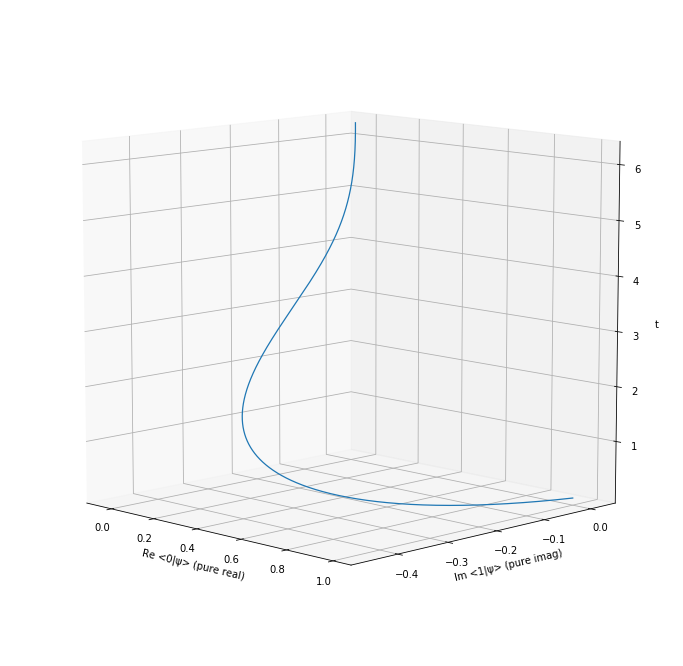
\includegraphics[width=0.45\linewidth]{2ldetect/3D-evol-cont.png}%
  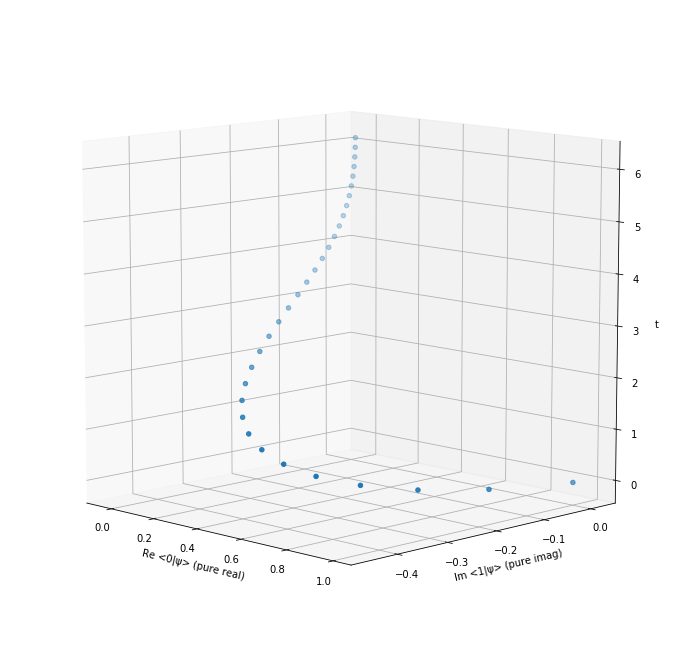
\includegraphics[width=0.45\linewidth]{2ldetect/3D-evol-pw.png}
  \captionof{figure}{
    \color{Green}
    Evolution of the qubit under the complex absorption potential, with loss of normalization.
    \textit{Left}: ``Schr\"odinger'' evolution. \textit{Right}: discrete PaW model with a 32-level clock.
  }
\end{center}\vspace{0.5cm}

Finally, as shown in \cite{RuschhauptAbsorption}, the detection probability amplitude
in time
can be derived applying the operator $\sqrt{2\hat{D}}$ to the normalization-lossy
evolved state. It is proven therein that the square modulus of the result is equal
to the loss of normalization which corresponds to absorption probability rate of the detector.

In the PaW model, the above, together with the \eqref{eq:energyfix},
can be formalized in a compact way for each eigenvector of $\mathbb{J}$:
\begin{equation}
  \dket{\tilde{\epsilon}} = e^{-i\epsilon\hat{T}} \ox \sqrt{2\hat{D}} \dket{\epsilon}
\end{equation}
and, by linearity, to each combination of the above. The square modulus of
each pair of components in this ``probability history'' will bring to the distribution
in Figure~\ref{fig:toa}.

\section*{Another example: 3-level system and weak absorption}

For small values of $\gamma$ in \eqref{eq:complexpot},
the distortion caused by the detector is negligible.
Therefore the PaW method can be used without including the imaginary term
(while it is necessary in ordinary quantum mechanics,
in lack of a universally accepted definition of a time-of-arrival observable).
On the other hand, detection is probable well \emph{after} the first cycle of the clock.
Therefore we need to consider the \emph{conditional} probability: provided that detection happens
within $(0, T)$, what is the probability (density) that it happens at time $t$?

A similar Bayesian rule is necessary to define time-of-arrival within the PaW framework
anyway \cite{Maccone:QMOT}.

\subsection*{The (sightly) non-unitary evolution of a qutrit}
With respect to the \eqref{eq:complexpot} we have chosen in this case:
\begin{equation}
  \hat{H} \repr \left[\begin{matrix}0 & 1 & 0\\1 & 0 & 1\\0 & 1 & 0\end{matrix}\right] \text{;} \quad
  \psi_0 \repr \left[\begin{matrix}\frac{\sqrt{2}}{2}\\\frac{1}{2} + \frac{i}{2}\\0\end{matrix}\right] \text{;} \quad
  \hat{D} = \left[\begin{matrix}0 & 0 & 0\\0 & 0 & 0\\0 & 0 & \gamma\end{matrix}\right] \text{,}
\end{equation}
with the order of $\gamma \approx 10^{-2}$.

A summary of the results is shown in the figures below.
\vspace{0.5cm}

\vspace{0.5cm}
\begin{center}
  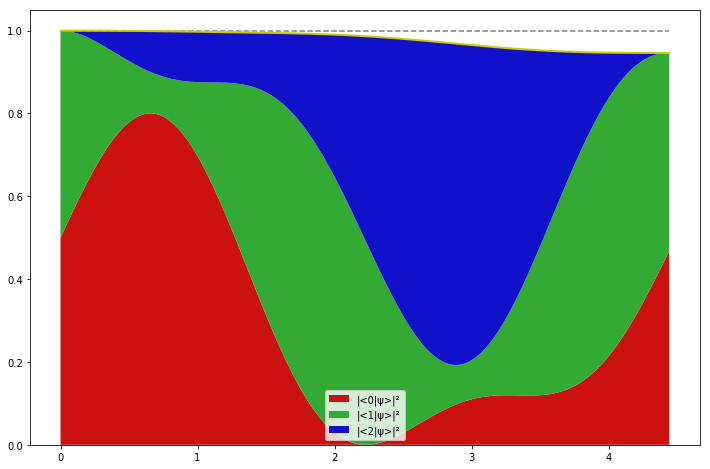
\includegraphics[width=0.6\linewidth]{2ldetect/qutrit-lossy.png}
  \captionof{figure}{
    \color{Green}
    Loss of normalization (small, but noticeable on top-right of the plot),
    and components of the qutrit,
    over the first cycle $t \in (0, \sqrt{2}\pi)$.
  }
\end{center}
\vspace{0.5cm}
\vspace{0.5cm}
\begin{center}
  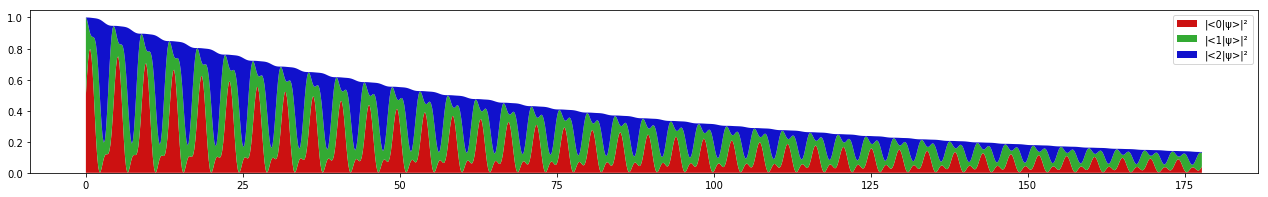
\includegraphics[width=\linewidth]{2ldetect/qutrit-lossy-long.png}
  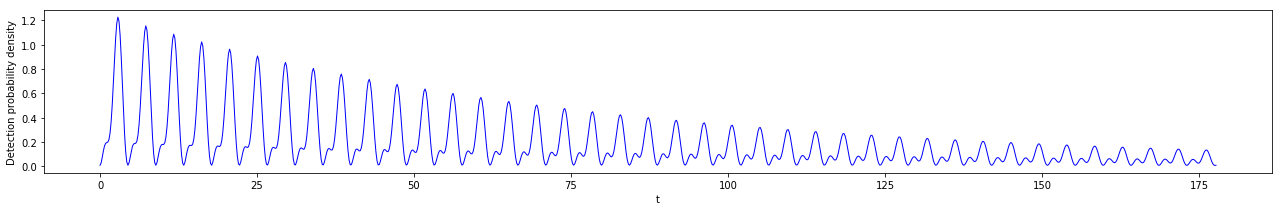
\includegraphics[width=\linewidth]{2ldetect/qutrit-lossy-long-detect.png}
  \captionof{figure}{
    \color{Green}
    Evolution (top) and time-of-arrival at state $\ket{2}$ (bottom) over a longer time.
  }
\end{center}
\vspace{0.5cm}
\vspace{0.5cm}
\begin{center}
  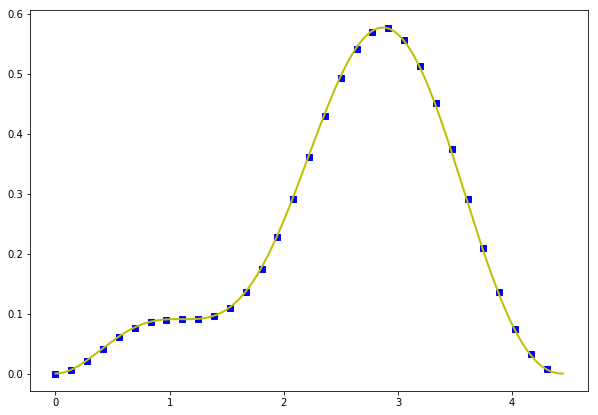
\includegraphics[width=0.6\linewidth]{2ldetect/qutrit-detect-both.png}
  \captionof{figure}{
    \color{Green}
    \emph{Discrete points:} time-of-arrival at $\ket{2}$ per (discrete) PaW model,
    using conditional definition of \cite{Maccone:QMOT} and no complex potential.
    \emph{Continuous line:}
    Detector model with complex potential (as in \cite{RuschhauptAbsorption}),
    and probability conditioned in the first cycle.
  }
\end{center}

%----------------------------------------------------------------------------------------
%	CONCLUSIONS
%----------------------------------------------------------------------------------------

\color{SaddleBrown} % SaddleBrown color for the conclusions to make them stand out


% \section*{Conclusions and Outlook}

% \begin{itemize}
% \item Pellentesque eget orci eros. Fusce ultricies, tellus et pellentesque fringilla, ante massa luctus libero, quis tristique purus urna nec nibh. Phasellus fermentum rutrum elementum. Nam quis justo lectus.
% \item Vestibulum sem ante, hendrerit a gravida ac, blandit quis magna.
% \item Donec sem metus, facilisis at condimentum eget, vehicula ut massa. Morbi consequat, diam sed convallis tincidunt, arcu nunc.
% \item Nunc at convallis urna. isus ante. Pellentesque condimentum dui. Etiam sagittis purus non tellus tempor volutpat. Donec et dui non massa tristique adipiscing.
% \end{itemize}

\color{DarkSlateGray} % Set the color back to DarkSlateGray for the rest of the content

\scriptsize

 %----------------------------------------------------------------------------------------
%	REFERENCES
%----------------------------------------------------------------------------------------

%\bibliographystyle{plain}
%\bibliography{bib/main}

%biblatex
\printbibliography

\end{multicols}
\end{document}
